\documentclass[10pt]{beamer}

\usetheme{metropolis}
\usepackage{appendixnumberbeamer}

\usepackage{booktabs}
\usepackage[scale=2]{ccicons}

\usepackage{pgfplots}
\usepgfplotslibrary{dateplot}

\usepackage{xspace}
\newcommand{\themename}{\textbf{\textsc{metropolis}}\xspace}


\usepackage{xcolor}
\usepackage{listings}
\usepackage{caption}
\DeclareCaptionFont{white}{\color{white}}
\DeclareCaptionFormat{listing}{%
	\parbox{\textwidth}{\colorbox{gray}{\parbox{\textwidth}{#1#2#3}}\vskip-4pt}}
\captionsetup[lstlisting]{format=listing,labelfont=white,textfont=white}
\lstset{frame=lrb,xleftmargin=\fboxsep,xrightmargin=-\fboxsep}

\lstset{
	% numbers=left,
	breaklines=true,
	% backgroundcolor=\color{light-gray},
	tabsize=4,
	% basicstyle=\ttfamily,
	literate={\ \ }{{\ }}1	
}


\title{Master Thesis Proposal}
\subtitle{Compliant Manipulation Using Task Specification and Reinforcement Learning}
\date{\today}
\author{Abhishek Padalkar}
\institute{Hochschule Bonn-Rhein-Sieg, Sankt Augustin}
% \titlegraphic{\hfill
\includegraphics[height=1.5cm]{logo.pdf}}

\begin{document}

\maketitle

\begin{frame}{Table of contents}
  \setbeamertemplate{section in toc}[sections numbered]
  \tableofcontents[hideallsubsections]
\end{frame}

\section{Introduction}

\begin{frame}[fragile]{Compliant Manipulation}
	\begin{itemize}
		\item Most of the real world robotic manipulation tasks present the need for compliant manipulation.
		\item Robot needs to respond to the contact forces while executing the task. 
		\item Classical planning and control algorithm fail to perform satisfactorily due to the lack of precise model of contact forces and high computational complexity.
	\end{itemize}
\end{frame}

\section{Problem Statement}

\begin{frame}{Problem Statement}
	
	\begin{itemize}
		\item We propose to create a framework based on task specification and model based reinforcement learning to solve the problem of compliant manipulation for given task in deterministic manner with fewer number of interactions with environment.
		\item We will evaluate our approach based by learning the task of opening door and cutting vegetables.
	\end{itemize}
\end{frame}

\section{Related Work}

\begin{frame}[fragile]{Task Specification in KRL}
	
	\begin{lstlisting}[label=KRL-sample,caption=KRL code]
		INI
		PTP HOME ; go to HOME joint configuration
		LIN P1   ; linear motion to point P1
		LIN P2	 ; linear motion to point P2
	\end{lstlisting}
	\begin{itemize}
		\item Heavily used in industrial settings 
		\item Reliable
		\item Difficult to integrate sensory feedbacks
		\item Limited expressive power \cite{leidner2017cognitive}
	\end{itemize}
\end{frame}

\begin{frame}[fragile]{Task Specification in Leidner's PhD work\cite{leidner2017cognitive}}
	\begin{itemize}
		\item Symbolic representation of the task in PDDL. 
		\item Geometric representation of the task specifies the sequence of low level movement sequences needed to complete the action. 
		\item Geometric representation only specifies discrete motion primitives and not the parametric representation of the motion primitives. 
		\item Actual parameterization and control is left to low level control module. 
	\end{itemize}
\end{frame}

\begin{frame}[fragile]{Task Specification by Meson et. al. \cite{mason1981compliance}}
	
	\begin{lstlisting}[label=tff,caption=Task Specification using TFF: Open Door]
		move compliantly {
			with task frame directions
			xt: force 0 N
			yt: force 0 N
			zt: velocity v mm/sec
			axt: force 0 Nmm
			ayt: force 0 Nmm
			azt: force 0 Nmm
		} until distance > d mm 
	\end{lstlisting}
	

\end{frame}

\begin{frame}
	\begin{itemize}
		\item Using hybrid control, various control modes are assigned to each axis of the \textit{task frame} or \textit{compliance frame}\cite{nagele2018prototype}. 
		\item This framework doesn't consider the specification of task or motion quality related parameters like velocity damping or instantaneous sensory inputs. 
		\item It also specify action to be executed \textit{compliantly} but does not specify the how? 
	\end{itemize}
\end{frame}

\begin{frame}{iTaSC}
	\begin{itemize}
		\item iTaSC developed in \cite{DeSchutter-ijrr2007, DecreBruyninckxDeSchutter2013, decre09}, synthesizes control inputs based on provided task space constraints. 
		\item It formulates a optimization problem considering provided constraints in the environment. 
		\item In case of conflicting constraints, constraints are weighted in the optimization problem.
		\item Suffers heavily by inaccurate  modeling of the constraints.  
	\end{itemize}
\end{frame}

\begin{frame}{Reinforcement Learning for Manipulation}
	\begin{itemize}
		\item In model free and model based reinforcement learning, an agent learns the skills by exploring the environment and adopting the parameters which governs the trajectory of the agent in the environment.
		\item Learning all the parameters of the policy can be computationally very expensive and might require large number of interactions with the environment.
		\item Large number trials causes wear and tear in mechanical parts and even damage to robot and the environment apart from being time consuming. 
		\item If we can model the environment and constraints on the motion of the robot, we can drastically reduce the number of parameters to be learn to achieve the task.
		\item Use of reinforcement learning to learn these reduced number of parameters can result in near optimal policy for achieving the task.
	\end{itemize}
\end{frame}

\begin{frame}{Reinforcement Learning for Manipulation}
	\begin{itemize}
		\item Manipulation tasks imply complex contact interactions with an unstructured environment and require a controller that is able to handle force interactions in a meaningful way \cite{kalakrishnan2011learning}.
		\item Planning algorithms would require precise dynamics models of the resulting contact interactions. 
		\item These models are usually unavailable, or so im-precise that the generated plans are unusable\cite{kalakrishnan2011learning}. 
		\item Kalakrishnan et. al. in \cite{kalakrishnan2011learning} proposed an intelligent control algorithm with reinforcement learning for opening door task.
		\item It considers the constraints on door motion greatly reducing, the number of parameters to be learned. 
	\end{itemize}
\end{frame}

\section{Proposed Solution}
\begin{frame}[fragile]
	We plan to solve a compliant manipulation task by providing task specification and then tuning the task parameters with the help of re-reinforcement learning.
	
	Examples of task modeling: 
	
	\begin{lstlisting}[label=open_door_ts,caption=Task specification for opening door]
	open_door
	{
		f_x = f(environment, robot, task)
		v_y = v1
		max_acc = a_max
		max_dec = a_dec
	}until(f(...))

	\end{lstlisting}
	
\end{frame}

\begin{frame}[fragile]
	
	\begin{lstlisting}[label=open_door_ts,caption=Task specification for cutting vegetables]
	open_door
	{
	f_z = f(environment, robot, task, v_x)
	v_x = g(t)
	max_acc = a_max
	max_dec = a_dec
	}until(f(...))
	
	\end{lstlisting}
	\begin{itemize}
		\item Force specification on compliant axis
	\end{itemize}
\end{frame}


\begin{frame}{Composition}
	\begin{figure}[!h]
		\center{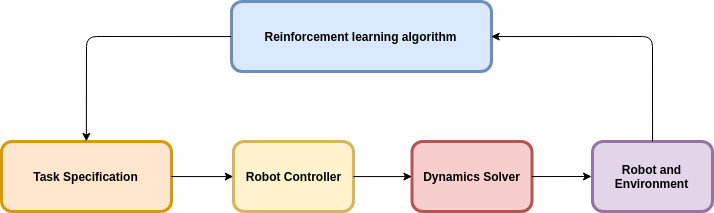
\includegraphics[width=\textwidth]
			{images/composition.png}}
		\caption{\label{fig:composition} Composition}
	\end{figure}
\end{frame}

\begin{frame}{Reinforcement Learning Algorithm to be Used}
	\begin{itemize}
		\item We plan to use Path Integral Policy Improvement algorithm for learning\cite{kalakrishnan2011learning}.
		\item $PI^{2}$ Algorithm is a probabilistic algorithm for policy improvement. 
		\item Multiple works so far has proven the capability of $PI^{2}$. 
	\end{itemize}
	The aim is to minimize the expected cost of each cycle which is given by:
	$$J(W) = c_{t} + \int_{t_{0}}^{t} (c_{i}(t)+\frac{1}{2} {W}^{T}RW)dt$$
	$c_{t}$ is terminal cost.
	$c_{i}(t)$ is instantaneous cost at instant $t$.
	$R$ is the weighting matrix, which minimizes control cost. $W$ is policy parameter matrix.
\end{frame}

\begin{frame}{Advantages}
	\begin{itemize}
		\item Task specification is a practical approach for solving manipulation.
		\item Scope for representing motions in multiple type of motion primitives. e.g. DMPs
		\item Reinforcement learning replaces the need of model accuracy.
		\item This approach will require less number of robot-environment interactions as compared to other reinforcement learning approaches.
		\item This solution bridges the gap between task specification approaches and learning methods fo compliant manipulation. 
	\end{itemize}
	
	
	
\end{frame}

\begin{frame}{Challenges}
	\begin{itemize}	
		\item Task specification and parameterization
		\item Design of reward function
		\item Safety of the robot
	\end{itemize}
\end{frame}

\begin{frame}[allowframebreaks]{References}

  \bibliography{../../project-proposal/bibliography}
  \bibliographystyle{abbrv}

\end{frame}

\end{document}
